\begin{section}{Mise en place d'un bootstrapping}
\begin{subsection}{Un point sur la sécurité}
	Nous avons vu que le système cryptographique que nous étudions est IND-CPA, ce qui est le niveau de sécurité
	théorique que l'on veut généralement. La première question qui se pose pour le bootstrapping est de savoir si
	il a la sécurité circulaire, expliquée dans la définition~\ref{def:circular}.
	Nous n'avons pas trouvé de démonstration de cette sécurité dans l'article original \cite{EPRINT:GenSahWat13} 
	ou encore dans d'autres expositions (comme \cite{halevi}). Nous devons donc la supposer pour cette section.
	cette hypothèse.
\end{subsection}
\begin{subsection}{Un premier découpage}
	Afin de pouvoir effectuer un bootstrapping à partir de l'algorithme de déchiffrement \textbf{Dec}, nous allons avoir besoin de l'exprimer uniquement à partir d'opérations \textbf{NAND} sur des 0 et des 1.
	
	La première clé secrète est un vecteur d'éléments de $\ZZq$, pas de \{0,1\}, ce qui signifie que pour pouvoir l'utiliser dans le bootstrapping, on est contraint de se servir des chiffrés de chaque bit de chaque élément de la clé.

	Pour cela, on considère qu'à tous les éléments de $\ZZq$ est associé une liste de $l-1$ éléments contenant son écriture en binaire.

\begin{lstlisting}
decrypt(C) :
	trouver $1 \leqslant i \leqslant l$ tel que $q/4 \leqslant 2^i < q/2$
	calculer $a = C_i \cdot \vec{v}$
	retourner $|\frac{a}{\vec{v}_i}|$
\end{lstlisting}

Notons que:

\begin{align*}
	C_i \cdot \vec{v} &= \sum_{j=0}^N C_{i,j} v_j \\
	&= \sum_{j=0}^N \sum_{k=0}^l \left( C_{i,j,k} 2^k \right) v_j \\
	&= \sum_{j=0}^N \sum_{k=0}^l C_{i,j,k} (2^k v_j)
\end{align*}

	Or, même lorsque l'algorithme se fait homomorphiquement, les valeurs
	$C_{i,j,k} \in \{ 0,1 \}$ sont connues. On réduit donc le problème de
	calculer un produit scalaire à celui de faire la somme d'au plus $l * N
	= \bnorm{q}^2 (n+1)$ vecteurs constitués de 0 et de 1.

	Nous allons maintenant voir comment décrire l'algorithme uniquement avec des portes \textbf{NAND}, et majorer la profondeurs en \textbf{NAND} de l'algorithme final.

	Comme nous utiliserons aussi les portes logiques \path{NO}, \path{AND}, \path{OR} et \path{XOR}, notons que:
\begin{itemize}
\item \path{NO}$(a) = \overline{a}$ se fait en un \textbf{NAND};
\item \path{AND}$(a, b) = a \land b$ se calcule en deux \textbf{NAND} et est de
	profondeur 2;
\item \path{OR}$(a, b) = a \lor b$ se fait en trois \textbf{NAND} et est de
	profondeur 2;
\item \path{XOR}$(a, b) = a \oplus b$ se calcule en six \textbf{NAND} et est de
	profondeur 4.
\end{itemize}
De plus, pour $f$ et $g$ des formules de profondeur de nand respectives $u$ et
$v$, notons que:
\begin{itemize}
\item $\overline{f}$ a une profondeur $u+1$;
\item $f \land g$ et $f \lor g$ ont une profondeur de $\text{max}(u,v) + 2$;
\item $f \oplus g$ a une profondeur de $\text{max}(u,v) + 4$;
\end{itemize}
\end{subsection}
\begin{subsection}{Sommer des vecteurs avec une profondeur en NAND minimale}

	Nous voulons pouvoir sommer homomorphiquement $nb$ nombres vus comme des listes de taille $s$ dont les éléments sont des chiffrés de 0 ou de 1 en minimisant la profondeur de NAND requise. 

	Pour cela, nous allons tout d'abord étudier deux opérations simples sur des listes.

\vspace{0.3cm}
\noindent
\textbf{basic\_sum : addition classique de deux listes :}
\paragraph{}
	Il s'agit de l'algorithme naïf de somme de deux nombres binaire, commençant par les bits de poids faible puis remontant vers les bits de poids plus élevés en conservant des retenues, sauf celle qui \og sort \fg des listes. On l'appellera ici \textbf{basic\_sum}. Soient 
\[ A = \sum_{i=0}^{s-1} a_i 2^i \quad B = \sum_{i=0}^{s-1} b_i 2^i\]
que l'ont veux sommer. La somme
\[D =\sum_{i=0}^{s-1} d_i 2^i\]
est alors définie par :
	
\begin{figure}[!h]
\begin{lstlisting}
$r_{-1}$ = 0
for $i$ in range($s$):
	$d_i$ = $a_i \oplus b_i \oplus c_{i-1}$
	$c_i$ = $(a_i \land b_i) \lor (c_{i-1} \land (a_i \lor b_i))$
\end{lstlisting}
\end{figure}

	Le problème de cette méthode est que la profondeur de NAND nécessaire explose du fait que la formule exprimant $d_{s-1}$ dépend de $a_0$ et $b_0$, et ce à cause de la récursivité du calcul des $c-i$.

	Calculer $d_i$ peut se faire en n'utilisant la retenue que pour un $\oplus$, ce qui n'ajoute que 4 à la profondeur en \textbf{NAND} du calcul. $c_i$ est calculé en appliquant un \path{AND} et un \path{OR} à $c_{i-1}$, ce qui ajoute aussi 4 à la profondeur. $c_0 = a_0 \land b_0$ et peut donc être trouvé avec une profondeur de 2 \textbf{NAND}.
	
	On obtient alors la proposition suivante :
\begin{prop}
	L'algorithme \textbf{basic\_sum} nécessite une profondeur de $4*s - 2$ \textbf{NAND}.
\end{prop}


	Il s'avère qu'il existe une méthode pour additionner deux vecteurs en $\mathcal{O}(\log(s))$, il s'agit du carry lookahead adder que nous présentons maintenant.

	\textbf{carry lookahead adder: addition de deux vecteurs avec une profondeur plus faible de NAND}

	Nous appelerons \textbf{cla\_sum} cet algorithme. Sa différence avec la somme classique est que les retenues sont en partie calculées en parallèle, ce qui permet via le passage à un arbre binaire de diminuer la profondeur de NAND utilisée.

	Bien que nous en avons vu plusieurs expositions, nous n'en avons pas trouvé qui donne précisément les formules à utiliser dans un cas général. Nous exposons donc ici le détail des formules et des démonstrations sur la profondeur en NAND.

	Notons que pour simplifier les formules, nous faisons ici commencer les indices de listes par 1.

	On suppose que les listes ont pour taille une puissance de deux $s = 2^u$. On pose alors, notant le OU logique par l'addition et le ET logique comme un produit :
\begin{align*}
	&{G1}_i = a_i b_i\quad {P1}_i = a_i + b_i \qquad \text{pour $1 \leqslant i \leqslant 2^u$} \\
	&{G2}_i = {G1}_{2i} + {G1}_{2i-1}{P1}_{2i} \qquad {P2}_i = {P1}_{2i-1} {P1}_{2i} \quad \text{pour $1 \leqslant i \leqslant 2^{u-1}$} \\
	&\cdots \\
	&{(G2^k)_{i}} = {(G2^{k-1})_{2i}} + {(G2^{k-1})_{2i-1}}{(P2^{k-1})_{2i}}\qquad {(P2^{k})_i} = {(P2^{k-1})_{2i-1}} {(P2^{k-1})_{2i}} \quad \text{pour $1 \leqslant i \leqslant 2^{u-k}$} \\
	&\cdots \\
	&{G2^u} = {(G2^{u-1})_{2}} + {(G2^{u-1})_{1}}{(P2^{u-1})_{2}}\qquad {P2^{u}} = {(P2^{u-1})_{1}} {(P2^{u-1})_{2}}
\end{align*}

	Les variables G sont dites variables de générations et celles avec un P sont
dites variables de propagations.

	On a alors la propriété suivante :
\begin{prop}
	Considérons $0 \leqslant k \leqslant u$ et $1 \leqslant i \leqslant 2^{u-k}$ et notons $B$ le bloc :
\[ (i-1)2^{k} + 1, \cdots, i 2^{k} \]
	On considère alors $a_{|B}$ et $b_{|B}$ les nombres binaires obtenus en restreignant les écritures binaires de $a$ et $b$ aux positions $B$. Alors, 
\begin{itemize}
\item $(G2^k)_i$ est vrai si et seulement si l'algorithme de somme binaire classique entre $a_{|B}$ et $b_{|B}$ crée une retenue à la dernière position, c'est à dire à la position\footnote{on commence à compter à partir de 1} $2^k$. On dit alors que le bloc $B$ génère une retenue.

\item $(P2^k)_i$ est vrai si et seulement si, considérant l'algorithme de somme binaire entre $a_{|B}$ et $b_{|B}$ où on ajoute une retenue à la position 1, il y a alors une retenue en dernière position. On dit alors que cette retenue s'est propagée le long du bloc $B$.
\end{itemize}
\end{prop}

\begin{proof}
	Procédons par récurrence. Pour $k = 0$, cela est facile : la somme de deux bits $u$ et $v$ ne produit une retenue que si $uv$ est vraie, et ne propage une retenue que si $u+v$ est vraie.

	Maintenant, observons les formules génériques :
\[{(G2^k)_i} = {(G2^{k-1})_{2i}} + {(G2^{k-1})_{2i-1}}{(P2^{k-1})_{2i}}\]
\[{(P2^{k})_i} = {(P2^{k-1})_{2i-1}} {(P2^{k-1})_{2i}} \]
pour le bloc
\[B = (i-1)2^k + 1, \cdots, i 2^k\]
	En notant $L$ et $R$ les deux moitiés de $B$ ($B = L|R$), on voit qu'elles peuvent s'interpréter ainsi :
\begin{itemize}
\item $(G2^k)_i$ n'est vrai que si $R$ génère une retenue ou bien si $L$ en génère une qui est propagée par $R$. Ce qui est équivalent à dire que $B$ génère une retenue.
\item $(P2^{k})_i$ n'est vraie que si une retenue arrivant au début du bloc $L$ est propagée et qu'une retenue arrivant au début du bloc $R$ est propagée. Ce qui, en composant les deux propagations, est équivalent à dire qu'une retenue arrivant au début du bloc $B$ est propagée.  
\end{itemize}
	On a donc bien ce qu'il fallait démontrer.
\end{proof}

\begin{prop} \label{g_et_p}
Le calcul de $(G2^k)_i$ a une profondeur en NAND de $2 + 4k$ et celui de $(P2^k)_i$ de $2 + 2k$.
\end{prop}

\begin{proof}
	La démonstration est directe par récurrence. 
\end{proof}

	Puis, pour un entier $a \in Z$, on défini les notations suivantes :
\begin{align*}
	&\nu(a) = \text{la plus petite puissance de 2 apparaissant dans l'écriture binaire de $a$}\\
	&\theta(a) = \text{le plus grand multiple de $2*\nu(a)$ inférieur à $a$}
\end{align*}

	Notons qu'alors : $a = \nu(a) + \theta(a)$. Par exemple :
\[\nu(6) = 2,\ \theta(6) = 4;\ \nu(13) = 1,\ \theta(13) = 12;\ \nu(12)= 4,\ \theta(12) = 8;\ \nu(1) = 1,\ \theta(1) = 0\]

\paragraph{}

	On définit alors les retenues $c_j$ par la formule :
\[c_j = {G\nu(a)}_{a/\nu(a)} + c_{\theta(a)} {P(\nu(a))}_{a/\nu(a)}\]
	où $c_0 = 0$ par définition.

	Voyons cela sur un exemple pour comprendre pourquoi cette formule fonctionne. Si on considère des vecteurs de taille $8 = 2^3$, les formules des retenues sont :
\begin{align*}
&c_1 = {G1_1} + c_0 {P1_1} = {G1_1} \\
&c_2 = {G2_1} + c_0 {P2_1} = {G2_1}  \\
&c_3 = {G1_3} + c_2 {P1_3}\\
&c_4 = {G4_1} + c_0 {P4_1} = {G4_1} \\
&c_5 = {G1_5} + c_4 {P1_5}\\
&c_6 = {G2_3} + c_4 {P2_3} \\
&c_7 = {G1_7} + c_6 {P1_7} \\
&c_8 = {G8_1} + c_0 {P8_1} = {G8_1} \\
\end{align*}

	Ainsi, si on veut additionner $a = 00111100$ et $b = 01010101$, on obtient :
\begin{center}
\begin{tabular}{llllllllll}
a  && 0&0&1&1&1&1&0&0 \\
b  && 0&1&0&1&0&1&0&1 \\
G1 && 0&0&0&1&0&1&0&0 \\
P1 && 0&1&1&1&1&1&0&1 \\
G2 && &0&&1&&1&&0 \\
P2 && &0&&1&&1&&0 \\
G4 && &&&1&&&&0 \\
P4 && &&&0&&&&0 \\
G8 && &&&&&&&0 \\
P8 && &&&&&&&0 \\
\end{tabular}
\end{center}

	et on trouve avec les formules précédentes :
\[ (c_1, ..., c_8) = (0,0,0,1,1,1,0,0) \]
	ce qui correspond bien aux retenues.

	On va maintenant voir que cette méthode est bien plus intéressante que la méthode classique concernant la profondeur de NAND.
\begin{prop}
	Pour deux vecteurs de taille $u$, calculer toutes les retenues nécessite une profondeur de moins de $8 \log(u) + 2$ NAND.
\end{prop}

\begin{proof}
	Notons $D(f)$ la profondeur et NAND d'une formule $f$, on a, pour tout $1 \leqslant j \leqslant 2^u $

\begin{align*}
D(c_j) &\leqslant 2 + \text{max}\left(2 + 4 \log(\nu(j)), 2 + \text{max}(D(c_{\theta(j)}), 2 + 2 \log(\nu(j)))\right) \\
&\leqslant 4 + \text{max}\left(2 + 4 \log(\nu(j)), D(c_{\theta(j)})\right) \\
& \leqslant 4 \log(u) + (2 + 4\log(u)) = 8 \log(u) + 2.
\end{align*}
La dernière inégalité utilise le fait que $D(c_0) = D(0) = 0$ et que la séquence $(j, \theta(j), \theta(\theta(j)), ...)$ devient constante à 0 en moins de $\log(u)$ étapes.
\end{proof}

	Une fois calculée les retenue, la somme entre deux listes $a$ et $b$ se fait comme la somme classique, avec : $r_i = a_i \oplus b_i \oplus c_i$.

	On en déduit donc :

\begin{thm}
	L'algorithme \textbf{cla\_sum} fait la somme de 2 vecteurs de taille $s$ avec une profondeur de moins de $8 \lceil \log(s) \rceil + 6$ NAND, donc en $\mathcal{O}(log(s))$.
\end{thm}

\begin{proof}
	Il suffit de compléter les vecteurs par des 0 pour se réduire au cas où la taille vaut $2^{\lceil \log(s) \rceil}$, on applique alors le travail fait précédemment.
\end{proof}

	Nous allons maintenant voire une autre opération permettant de diminuer encore la profondeur de NAND nécessaire pour sommer plus de 2 listes. 
\vspace{0.3cm}
\noindent
\textbf{reduced\_sum :}
\paragraph{}

	Soie
\[A = \sum_{i=0}^{s-1} a_i 2^i, \quad B = \sum_{i=0}^{s-1} b_i 2^i, \quad C = \sum_{i=0}^{s-1} c_i 2^i. \]
\textbf{reduced\_sum} va créer deux nombres qu'on nomme $X = \sum_{i=0}^{s-1} x_i 2^i$  et $Y = \sum_{i=0}^{s-1} y_i 2^i$ tels que $A + B + C = X + Y$.

	Ils se construisent ainsi, avec la convention que pour tout vecteur v, $v_i = 0 \  \forall \, i \not\in \llbracket 0, s-1 \rrbracket$ :
\begin{figure}[!h]
\begin{lstlisting}
for $i$ in range($s$):
	$x_i$ = $a_i \oplus b_i \oplus c_i$
	$y_i$ = $\overline{(\overline{a_{i-1}} \land \overline{b_{i-1}}) \oplus
	(\overline{b_{i-1}} \land \overline{c_{i-1}}) \oplus
	(\overline{a_{i-1}} \land \overline{c_{i-1}})}$
\end{lstlisting}
\end{figure}

	On remarque qu'ici, les coordonnées des résultats ne dépendent que des coordonnées voisines. La profondeur totale en NAND sera donc le max de la profondeur du calcul de $x_i$ et de celle du calcul de $y_i$.
	
	Calculer $x_i$ consiste en deux $\oplus$ successifs dont le deuxième utilise le résultat du premier. La profondeur en \textbf{NAND} est donc de 8. La profondeur maximale du calcul de $y_i$ est celle des éléments impliqués dans deux $\oplus$. Ces éléments subissent donc deux \path{NO}, un \path{AND} et deux \path{XOR}, atteignant ainsi une profondeur de 12 \textbf{NAND}.

\begin{prop}
	L'algorithme \textbf{reduction\_sum} nécessite une profondeur de $12$ \textbf{NAND}.
\end{prop}

	On comprend donc que pour sommer plusieurs listes, nous avons tout
	intérêt à utiliser \textbf{reduced\_sum} jusqu'à qu'il ne reste plus
	que deux listes, puis à utiliser \textbf{cla\_sum}, mais comment organiser ces "additions" de façon à minimiser la profondeur totale ?

\vspace{0.3cm}
\noindent
\textbf{organiser la somme des $nb$ listes :}
\paragraph{}
	L'algorithme naïf consisterai dans le premier cas à appliquer
	\textbf{cla\_sum} à deux listes puis à l'appliquer à chaque fois au
	résultat de la dernière somme avec une autre liste. Les deux variables
	additionnées lors de la première addition serait impliquées dans
	chacune	des $nb-1$ opérations et la profondeur en \textbf{NAND} serait
	donc de $(nb-1)(8\lceil\log(s)\rceil + 6)$.
	
\paragraph{}
	Dans le cas de \textbf{reduced\_sum}, l'algorithme naïf consisterai en
	: appliquer \textbf{reduced\_sum} à trois des listes à additionner,
	puis en choisir une autre et appliquer \textbf{reduced\_sum} à cette
	dernière accompagnée des deux listes précédemment retournée par
	\textbf{reduced\_sum} et ainsi de suite, jusqu'à ce qu'il ne reste plus
	de liste à ajouter au dernier résultat. On y applique alors \textbf{cla\_sum}. On atteint ainsi une profondeur de 
	$12(nb - 2) + 8 \lceil \log(s) \rceil + 6 = 12 nb + 8 \lceil \log(s)
	\rceil - 18$ \textbf{NAND}.
	
\paragraph{}
	Les additions peuvent cependant être bien mieux ordonnées :
	
	Par exemple, en visualisant l'organisation comme un arbre, un arbre
	équilibré réduit au maximum la profondeur et permet à de sommer les
	$nb$ listes en utilisant uniquement \textbf{basic\_sum} avec une
	profondeur en \textbf{basic\_sum} de $\log_2(nb)$. On obtient donc une
	profondeur en \textbf{NAND} en $\mathcal{O}(\log(nb) * (8\log(s) + 6))
	= \mathcal{O}(\log(s) * \log(nb))$ et non plus en $\mathcal{O}(s * nb)$.

	Si l'on construit un équivalent pour \textbf{reduced\_sum}, toujours en
	terminant par un \textbf{cla\_sum}, on obtient une profondeur en
	\textbf{NAND} en $\mathcal{O}(\log(nb) + \log(s))$.

\begin{prop}
	Il est possible de sommer $\text{nb}$ vecteurs de $s$ éléments avec une profondeur de $4s + 36\log_3(nb) -22$ \textbf{NAND}.
\end{prop}

\begin{proof}
	Soit $p \geqslant 3$ tel que $3^{p-1} < nb \leqslant 3^{p}$.
	
	En réunissant les listes à notre disposition par groupes de 3 et en leur appliquant \textbf{reduced\_sum}, puis en recommançant deux fois on se retrouve avec au plus $8 * 3^{p-3} < 3^{p-1}$ listes à sommer.
	
	On peut donc se ramener à $nb' \leqslant 9$ avec une profondeur en \textbf{reduced\_sum} de $3(p - 2)$.
	
	De là, on peut calculer la somme totale avec une profondeur de quatre \textbf{reduced\_sum} et un \textbf{basic\_sum} :

\center
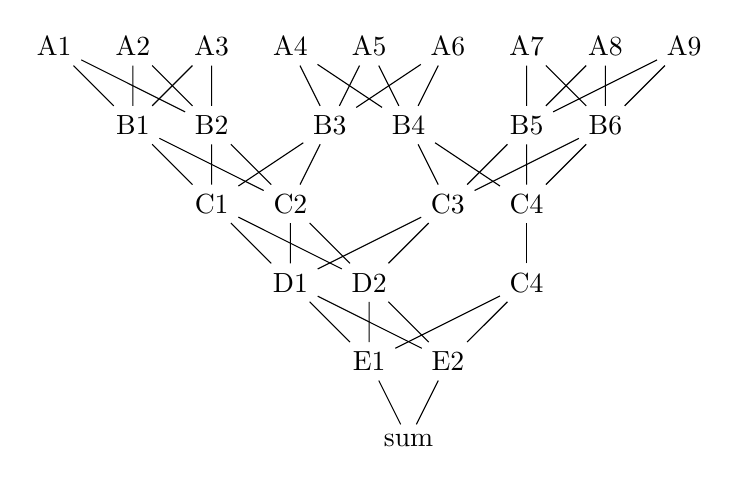
\begin{tikzpicture}
\node (A1) at (0,0) {A1};
\node (A2) at (1,0) {A2};
\node (A3) at (2,0) {A3};
\node (A4) at (3,0) {A4};
\node (A5) at (4,0) {A5};
\node (A6) at (5,0) {A6};
\node (A7) at (6,0) {A7};
\node (A8) at (7,0) {A8};
\node (A9) at (8,0) {A9};

\node (B1) at (1,-1) {B1};
\node (B2) at (2,-1) {B2};
\node (B3) at (3.5,-1) {B3};
\node (B4) at (4.5,-1) {B4};
\node (B5) at (6,-1) {B5};
\node (B6) at (7,-1) {B6};

\draw (B1) --(A1) --(B2);
\draw (B1) --(A2) --(B2);
\draw (B1) --(A3) --(B2);
\draw (B3) --(A4) --(B4);
\draw (B3) --(A5) --(B4);
\draw (B3) --(A6) --(B4);
\draw (B5) --(A7) --(B6);
\draw (B5) --(A8) --(B6);
\draw (B5) --(A9) --(B6);

\node (C1) at (2,-2) {C1};
\node (C2) at (3,-2) {C2};
\node (C3) at (5,-2) {C3};
\node (C4) at (6,-2) {C4};

\draw (C1) --(B1) --(C2);
\draw (C1) --(B2) --(C2);
\draw (C1) --(B3) --(C2);
\draw (C3) --(B4) --(C4);
\draw (C3) --(B5) --(C4);
\draw (C3) --(B6) --(C4);

\node (D1) at (3,-3) {D1};
\node (D2) at (4,-3) {D2};
\node (D3) at (6,-3) {C4};

\draw (D1) --(C1) --(D2);
\draw (D1) --(C2) --(D2);
\draw (D1) --(C3) --(D2);
\draw (D3) --(C4);

\node (E1) at (4,-4) {E1};
\node (E2) at (5,-4) {E2};

\draw (E1) --(D1) --(E2);
\draw (E1) --(D2) --(E2);
\draw (E1) --(D3) --(E2);

\node (sum) at (4.5,-5) {sum};

\draw (E1) --(sum) --(E2);
\end{tikzpicture}

	On obtient ainsi une profondeur totale en \textbf{NAND} de $8 \lceil
	\log(s)\rceil +
	6+
	12(3p - 2) = 8 \lceil \log(s) \rceil + 36p -18$. Or, par définition, $p = \lceil \log_3(nb)
	\rceil$ donc on a bien une profondeur en \textbf{NAND} de $8 \lceil
	\log(s) \rceil +
	36\lceil\log_3(nb)\rceil -18$.
\end{proof}

\end{subsection}
\begin{subsection}{Prendre la valeur absolue dans $\ZZq$}
	Rappelons que la valeur absolue d'un élément $x\in \ZZq$ est par définition la valeur absolue de son représentant dans $\rrbracket -q/2, q/2\rrbracket$. 
	
	Dans notre situation, $q = 2^l$ et nous représentons $a\in \ZZq$ par une liste de taille\footnote{Pour des raisons techniques, il est en fait représenté par une liste de taille $l$, mais nous ne faisons alors pas attention au dernier bit} $l-1$, le bit de poids faible étant à gauche. Autrement dit :
\[ a = [a_0, ..., a_{l-1}] \quad \text{pour représenter } a = \sum_{i=0}^{l-1} a_i 2^i\]

	On peut alors calculer en binaire la valeur absolue de $a$ ainsi :

\vspace{0.5cm}
\begin{lstlisting}
if $a_{l-1} = 0$: 
	# on a $a < q/2$
	return $a$
else:
	# on a $a < q/2$, alors $|a - q| = \left( (2^l - 1) - a + 1 \right)$
	$a$ = [NOT($a_i$) for $i$ in range($l$)]
	return basic_sum($a$, $1$)
\end{lstlisting}

	Toutefois, il n'est pas possible de faire de conditions homomorphiquement avec ce système, aussi, afin de pouvoir l'écrire homomorphiquement, on va en fait considérer le code suivant:

\vspace{0.5cm}
\begin{lstlisting}
$b$ = basic_sum([NOT($a_i$) for $i$ in range($l$)], 1)
return [($a_{l-1} \land a_i) \lor (\overline{a_{l_1}} \land b_i)$  for $i$ in range($l$)]
\end{lstlisting}

	On peut alors utiliser les comptes déjà fait, notamment concernant la profondeur en \textbf{NAND} de \textbf{basic\_sum}, pour conclure :

\begin{prop}
	En conservant nos conventions pour la représentation des données,
	prendre la valeur absolue d'un élément $a\in \ZZq$ demande une
	profondeur de moins de $8\lceil \log(s) \rceil + 11$ \textbf{NAND}.
\end{prop}
En additionnant nos différents comptes, on peut alors conclure sur la
profondeur de NAND nécessaire.
\begin{thm} \label{size_dec}
	Si $q$ est une puissance de $2$.
	On peut effectuer 
	l'algorithme \textbf{Dec} avec une profondeur de NAND plus petite que
	\[88 \lceil \log(\log(q)) \rceil + 36 \log\left(n)\right) \]
	et donc, en $O(\log(n) + \log(\log(q)))$
\end{thm}
\begin{proof}
En utilisant les propositions précédentes ainsi que le fait qu'il y a au plus $N*l = \log(q)^2 * (n+1)$ vecteurs de
sommés, on obtient une majoration de la profondeur de NAND par:
\[16 \lceil \log(\log(q)) \rceil + 36 \log_3\left(\log(q)^2
*(n+1)\right) = 16 \lceil \log(\log(q)) \rceil + 72 \log_3(\log(q)) + 36 \log_3\left((n+1)\right) \]
et on majore le logarithme en base $3$ par celui en base $2$ pour conclure, en
utilisant aussi que $\log_3(n+1) \leq \log(n)$ (dés $n \geq 2)$.
\end{proof}
\end{subsection}
\begin{subsection}{Choix asymptotique de paramètres pour GSW avec bootstrapping}

On va utiliser l'inégalité grossière :
\[
88 \lceil\log(\log(q))\rceil + 36 \log(\log(n)) \leq 90\left(\log(\log(q)) + \log(n)\right) \]
pour voir qu'on aura un GWS avec bootstrapping si on peut évaluer des chemins
de profondeur
\[ L = 90 \left(\log(\log(q)) + \log(n)\right) \]

On avait dans la section \ref{param_leveled} vu qu'on pouvait avoir une
profondeur de $L$ NAND si on avait: 
\begin{equation}
q > 16 {(1+N)}^{L+2}
\end{equation}
En injectant la valeur précédente de $L$ et avec une autre majoration
grossière, on voit qu'il suffit d'avoir
\begin{equation}
q > {\left((n+1)(\lceil \log(q) \rceil + 1 )\right)}^{90 \left(\log(n) +
\log(\log(q))\right)}
\end{equation}

en suivant le raisonnement de Shai Halevi, on remarque 
que pour un $\rho > 90$ assez grand, il suffit d'avoir:

\begin{equation}
q > {\left(n\log(q))\right)}^{\rho \left(\log(n) + \log(\log(q))\right)}
\end{equation}
En utilisant l'hypothèse  \ref{hyp_dwle_boot} (page \pageref{hyp_dwle_boot}), notre jeu de contraintes est alors:

\[ \begin{cases}
\alpha  = n /q
	q = 2^\text{polylog$(n)$}\\ 
	m = 2(N + \bnorm{q}) \\  
	q > {\left(n\log(q))\right)}^{\rho \left(\log(n) + \log(\log(q))\right)}
	\end{cases} \]

On utilise alors une légère modification des paramètres conseillées par Shai Halevi:
\begin{thm}
Sous l'hypothèse de sécurité circulaire ainsi que l'hypothèse \ref{hyp_dlwe_boot} de difficulté de DWLE, les paramètres suivants rendent cryptosystème GSW bootstrapable et IND-CPA:

\[ \begin{cases}
 	n = \lambda \\
	q = \lceil n^{\rho \log^2(n)}\rceil \\
	m = 2(N + \bnorm{q}) \\  
	\alpha = n/q = 2^{\Theta(\log^2(n))}
	\end{cases} \]
\end{thm}
\begin{proof}
Il nous faut montrer que l'inégalité 
	\[ q > {\left(n\log(q))\right)}^{\rho \left(\log(n) +
	\log(\log(q))\right)} \]
est vérifiée pour $n$ assez grand.

L'inégalité est vérifiée si:

	\begin{align*} &n^{\rho \log^2(n)} > {\left(n\log(q))\right)}^{\rho \left(\log(n) +
	\log(\log(q))\right)}\end{align*}
qui devient, en passant au logarithme:
\[ 4 \log^3(n) > {(\log(n) + \log(\log(q)))}^2 \]

or,
\[ \log(\log(q)) < \log(\rho \log^3(n)) = \log(\rho) + 3 \log(\log(n)) \]
Il suffit donc de montrer que:
\[ \log^3(n) > {(\log(\rho) + 3\log(\log(n)) + \log(n))}^2 \]
qui est vrai pour $n$ assez grand.
\end{proof}
\begin{rmq}
Notons qu'il n'y a pas eu beaucoup de marge pour que les contraintes soient
respectée. Elles n'auraient par exemple pas été respectées si l'addition 
classique avait été utilisée à la place de l'addition avec carry lookahead.
\end{rmq}


\end{subsection}
\end{section}
